\chapter{Merging with Agriculture Dataset}

Imagine you are a farmer or an agricultural planner trying to make the best decisions for the upcoming planting season. What if you could peek into the climate’s behavior — temperature changes, rainfall patterns, wind speed — and understand exactly how these factors affect crop growth?

In this chapter, we take a fascinating step forward: we merge agricultural data with climate data. By combining these two worlds, we can uncover deeper insights about how weather and climate influence agricultural productivity, helping farmers, scientists, and policymakers make smarter, data-driven decisions. Let’s think about this together:

\begin{itemize}
    \item How do you think temperature fluctuations affect crop yield?
    \item What role does rainfall play in the growth cycle of different crops?
    \item Can wind patterns influence soil erosion or pollination?
\end{itemize}

By the end of this chapter, you’ll not only learn how to merge these datasets technically, but also explore why this integration is so crucial for understanding the bigger picture of agriculture under changing climate conditions.

Ready to see the magic happen when data meets reality? Let’s dive in!

\subsection*{Sourcing Agricultural Data}
To carry out this integration, we sourced agricultural data from a publicly available interactive visualization platform: \\
\href{https://public.tableau.com/app/profile/sadichchha1369/viz/NepaCropMapwithprovinceSAMPLE_15636442141840/Dashboard1}{Tableau Public - Nepal Crop Map Dashboard}\\
This dataset includes district-level agricultural information, which we align with our climate dataset to explore temporal and spatial patterns in greater depth.
But before merging, let’s take a step back. Data, especially from real-world sources is rarely perfect. It often contains missing entries, inconsistent formats, or irrelevant information. That’s why our first task is to clean the agricultural dataset to ensure it aligns smoothly with our climate data.


\section{Data Preprocessing}

Data preprocessing is the process of preparing raw data for analysis by cleaning and transforming it into a usable format. In data mining it refers to preparing raw data for mining by performing tasks like cleaning, transforming, and organizing it into a format suitable for mining algorithms.

Goal is to improve the quality of the data, handling missing values, removing duplicates, and normalizing data to ensures the accuracy and consistency of the dataset.

\subsection{Data Cleaning}

In this step, we focus on cleaning the dataset to prepare it for analysis.

\begin{enumerate}
\item \textbf{Check For Null Values:}

We should identify any missing values across the dataset, and decide how to handle them (impute, drop, or analyze separately). For this particular dataset no null values were found.

\begin{verbatim}
sum(is.na(df_climate))
\end{verbatim}

\item\textbf{Drop the unnecessary columns:}

In our data set the first column consisting of an index is not necessary so we can drop the first unnamed column from our climate dataset.

\begin{verbatim}
df_climate$X <- NULL
\end{verbatim}

\item\textbf{Inspect the Duplicate Columns:}

We must also check for duplicate columns and remove them as they don't provide any additional information. For this particular climate dataset no such columns were found.

\begin{verbatim}
duplicated(colnames(df_climate))
\end{verbatim}

\item\textbf{Convert Date Column to Date Format:}

Since the Date column is currently in character format, convert it to Date using \texttt{as.Date()}.

\begin{verbatim}
df_climate$Date <- as.Date(df_climate$Date, format = "%Y-%m-%d")
\end{verbatim}

\item \textbf{Set Date as Index:}

Setting the date as an index is not strictly necessary in R for time series data analysis, but it is often a good practice and can simplify time-based operations. Setting the date as an index (or primary column) helps in slicing, filtering, and aggregating data by time periods. For this data set I used \texttt{tsibble} package.

\begin{verbatim}
# Convert tibble to tsibble
df_climate <- as_tsibble(df_climate, index = Date, key = District)

# Check for index
index_name <- index_var(df_climate)
print(index_name)
\end{verbatim}

The dataset structure after cleaning looks like:

\begin{verbatim}
glimpse(df_climate)
\end{verbatim}

% Figure here ---------------------------
\begin{figure}[h!]
    \centering
    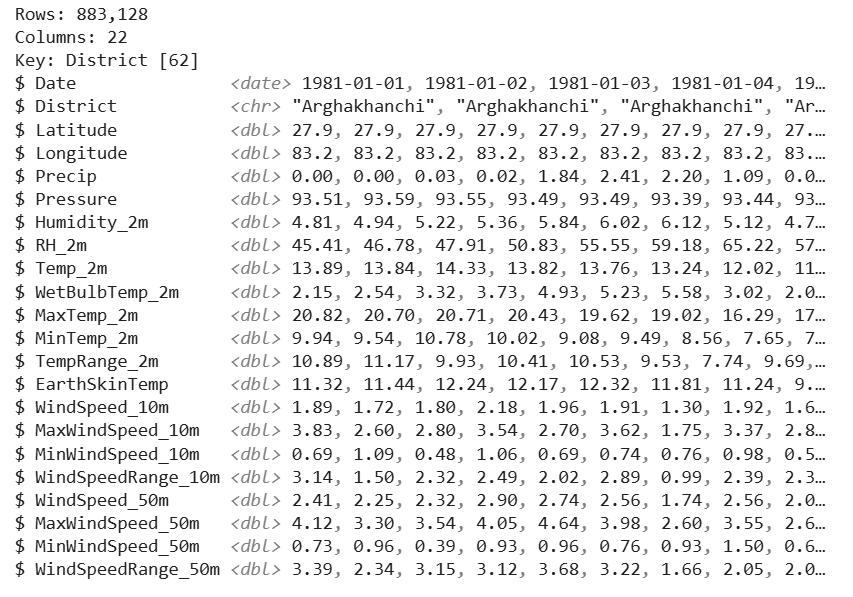
\includegraphics[width=0.6\textwidth]{figures/glimpse.png}
    \caption{Glimpse of the Cleaned Climate Dataset.}
\end{figure}

\end{enumerate}
\subsection{Feature Engineering}

Feature engineering is the process of taking raw data and transforming it into meaningful inputs that help a machine learning model understand patterns better. Think of it like preparing ingredients before cooking like when you chop, mix, and season them so the final dish tastes great.

In data analysis, this means creating new variables, cleaning data, selecting important information, or combining features to improve the model’s ability to make accurate predictions. Good feature engineering can often make a bigger difference in model performance than just using more complex algorithms.

It helps to create new features that might be helpful for your analysis. For this dataset, we can derive the month column from Date. Since Date is in format YYYY-MM-DD, we can extract the month and create a new column called month number. We can also create another column called month label and assign the names of the month (e.g., 1 = Jan, 2 = Feb, and so on).

\begin{verbatim}
# Extract month as number and label
df_climate$Month_Number <- month(df_climate$Date)     
df_climate$Month_Label <- month(df_climate$Date, label = TRUE)
\end{verbatim}

We can categorize the months into season and create a new column called “Season” for seasonal data analysis in the following way:

\begin{verbatim}
# Categorize months into seasons
df_climate <- df_climate %>%
  mutate(Season = case_when(
    month(Date) %in% c(12, 1, 2)  ~ "Winter",
    month(Date) %in% c(3, 4, 5)   ~ "Spring",
    month(Date) %in% c(6, 7, 8)   ~ "Summer",
    month(Date) %in% c(9, 10, 11) ~ "Fall"
  ))
\end{verbatim}

In R we can use \texttt{dplyr} and \texttt{lubridate} to extract the components of date. The function called \texttt{mutate()} can be used for creation of new columns and modifying the existing columns in our case.

\section{Merging Agriculture Data with Climate Data}

Previously, in the data slicing chapter, we created a subset of the climate dataset that includes only the districts classified as hilly regions. In this section, we will use this filtered climate data to merge with the agriculture dataset and perform agricultural analysis focused on the hilly region.

\subsection*{Filtering Hilly Region Data}
We first create a vector containing the list of districts in the hilly region:

\begin{verbatim}
districts_to_filter <- c("Arghakhanchi", "Baglung", "Baitadi", "Bhaktapur",
"Chitwan", "Dadeldhura", "Dailekh", "Dhading","Dhankuta", "Dolpa","Gorkha",
"Gulmi", "Ilam", "Jumla", "Kabhre", "Kaski", "Kathmandu", "Lalitpur",
"Lamjung", "Makwanpur", "Myagdi", "Nuwakot","Okhaldhunga","Palpa","Parbat",
"Rukum", "Salyan", "Sindhuli", "Surkhet", "Syangja")
\end{verbatim}

Then, we filter the climate dataset to include only the records corresponding to these districts:

\begin{verbatim}
filtered_hilly_data <- subset(df_climate, District %in% districts_to_filter)
\end{verbatim}

\subsection*{Extracting the Year from the Date Column}
Before merging the datasets, we need to extract the \texttt{Year} from the \texttt{Date} column in the filtered climate data:

\begin{verbatim}
filtered_hilly_data$Year <- year(filtered_hilly_data$Date)
\end{verbatim}

\subsection*{Saving the Filtered Dataset}
After filtering and extracting the year, we save the filtered dataset as a CSV file for future use:

\begin{verbatim}
write.csv(filtered_hilly_data,row.names = FALSE,file ="dataframe_hilly.csv")
\end{verbatim}

\subsection*{Merge Criteria}
To ensure proper alignment of the datasets, we merge them based on the following common identifiers:
\begin{itemize}
    \item \textbf{District:} The administrative region where both agricultural and climate data were recorded.
    \item \textbf{Year:} The calendar year of the recorded observations.
\end{itemize}

\subsection*{Merging the Datasets}
We merge the agricultural dataset \texttt{data\_agri\_clean} with the filtered hilly region climate dataset \texttt{filtered\_hilly\_data} based on the common identifiers:

\begin{verbatim}
merged_data <- merge(data_agri_clean, filtered_hilly_data, 
by = c("District", "Year"), all = FALSE) 
\end{verbatim}

This command performs an inner join, ensuring that only records with matching \texttt{District} and \texttt{Year} from both datasets are retained.

\section{Data Analysis and Visualization}

\subsection*{Identifying Major Crops in Hilly Regions}

This section identifies the main crops grown in Nepal’s hilly districts. By merging the cleaned agriculture and climate datasets, we analyze total crop production over time. Grouping by crop and summing production across years helps highlight the most widely produced crops in these regions.


\begin{verbatim}
top_crops <- merged_data %>%
  group_by(Crop) %>%
  summarise(Total_Production = sum(Production, na.rm = TRUE)) %>%
  arrange(desc(Total_Production))
ggplot(head(top_crops, 10), aes(
  x = Total_Production,y = reorder(Crop, Total_Production) )) +
geom_col(fill = "steelblue") + coord_flip() +
labs(title = "Top 10 Crops by Total Production in Hilly Regions",
x = "Crop", y = "Total Production")
\end{verbatim}

% Figure here-----------------------------
\begin{figure}[h]
\centering
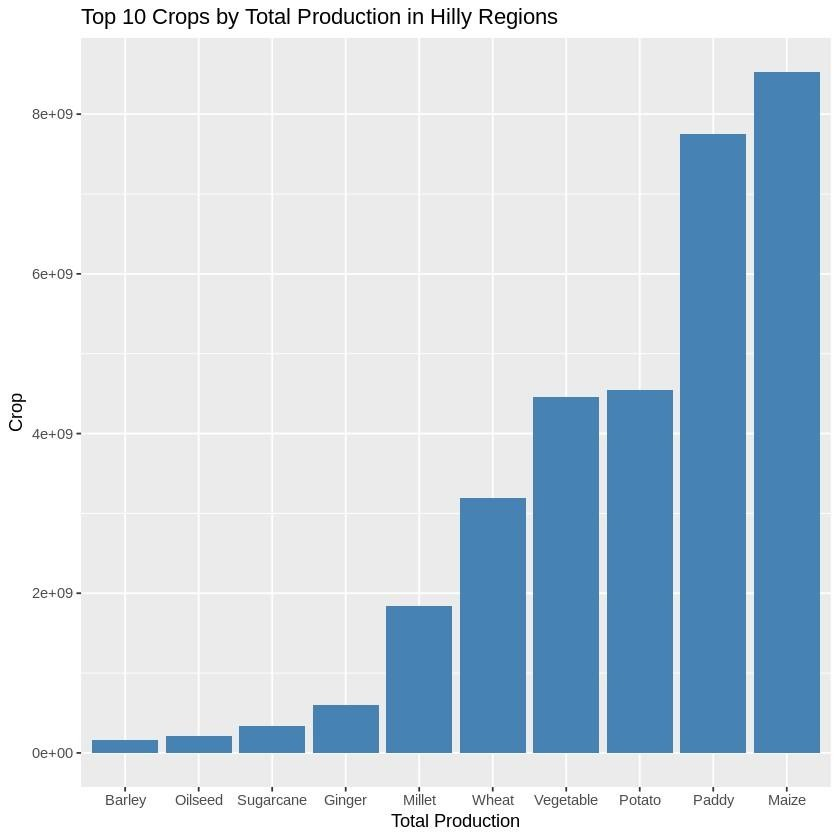
\includegraphics[width=0.5\textwidth]{figures/bar_agri.jpg}
\caption{ Top 10 Crops by Total Production in Hilly Region}
\end{figure}

The resulting plot clearly highlights the dominant crops cultivated in Nepal’s hilly regions. This insight is particularly valuable for stakeholders aiming to understand regional agricultural strengths or to design policies that support the most productive crops in these areas. Maize and Paddy are highly cultivated compared to others in hilly region.

\subparagraph*{Visualization of Agricultural Production by Crop Type in Hilly Districts
}
To understand the overall composition of agricultural production in the hilly districts, we visualize how different crop types contribute to production across various districts. This is done using a stacked bar chart, where each bar represents a district, and the stacked segments represent crop types.

\begin{verbatim}
ggplot(merged_data, aes(x = District, y = Production, fill = Crop.Type)) +
  geom_bar(stat = "identity", position = "stack") +
  coord_flip()
\end{verbatim}

% Figure here-----------------------------
\begin{figure}[h]
\centering
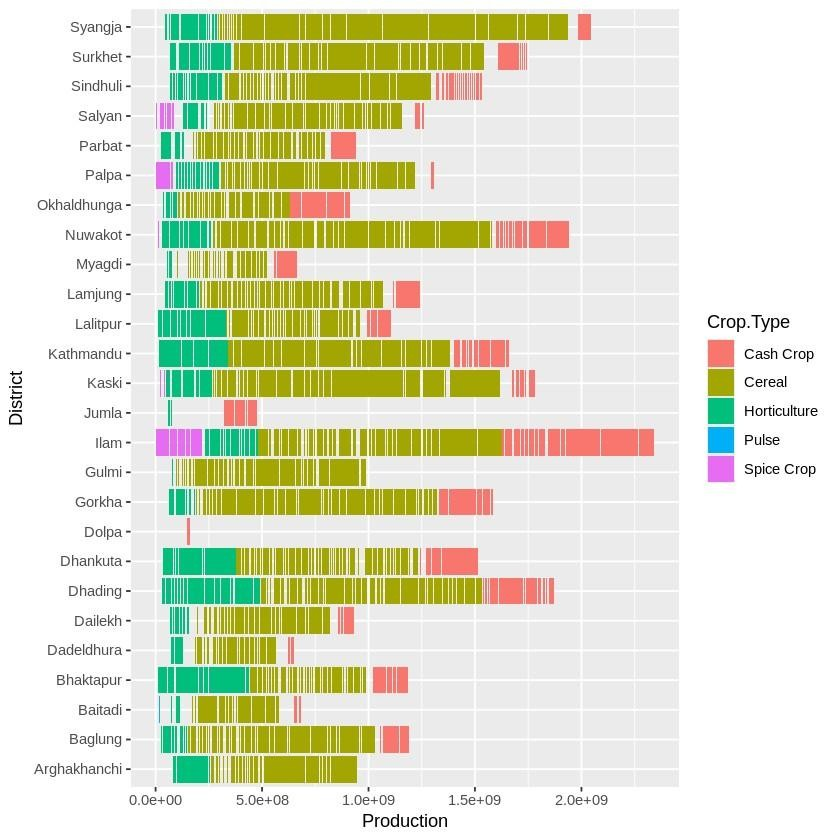
\includegraphics[width=0.6\textwidth]{figures/stacked_agri.jpg}
\caption{Stacked Barchart with crop type production in different districts}
\end{figure}

This visualization helps us compare which crop types dominate production in each district, and whether some regions have a more diverse agricultural profile than others. From the chart we can we that cereal production is highly dominating over hilly region.

\subsection*{Trend Analysis Over Time for Top 5 Crops}

To analyze how production of the most significant crops has changed over time in the hilly regions, we summarize and visualize the yearly production trends for the top 5 crops.

\begin{verbatim}
# Summarize yearly production for top crops
top_crops_list <- head(top_crops$Crop, 5)  # top 5 crops
yearly_trends <- merged_data %>%
  filter(Crop %in% top_crops_list) %>%
  group_by(Year, Crop) %>%
  summarise(Yearly_Production = sum(Production, na.rm = TRUE))
# Plot
ggplot(yearly_trends, aes(x = Year, y = Yearly_Production, color = Crop)) +
  geom_line(linewidth = 1) +
  labs(title = "Yearly Production Trends for Top Crops in Hilly Regions",
       x = "Year",
       y = "Production") +
  theme_minimal()
\end{verbatim}

% Figure here-----------------------------
\begin{figure}[h]
\centering
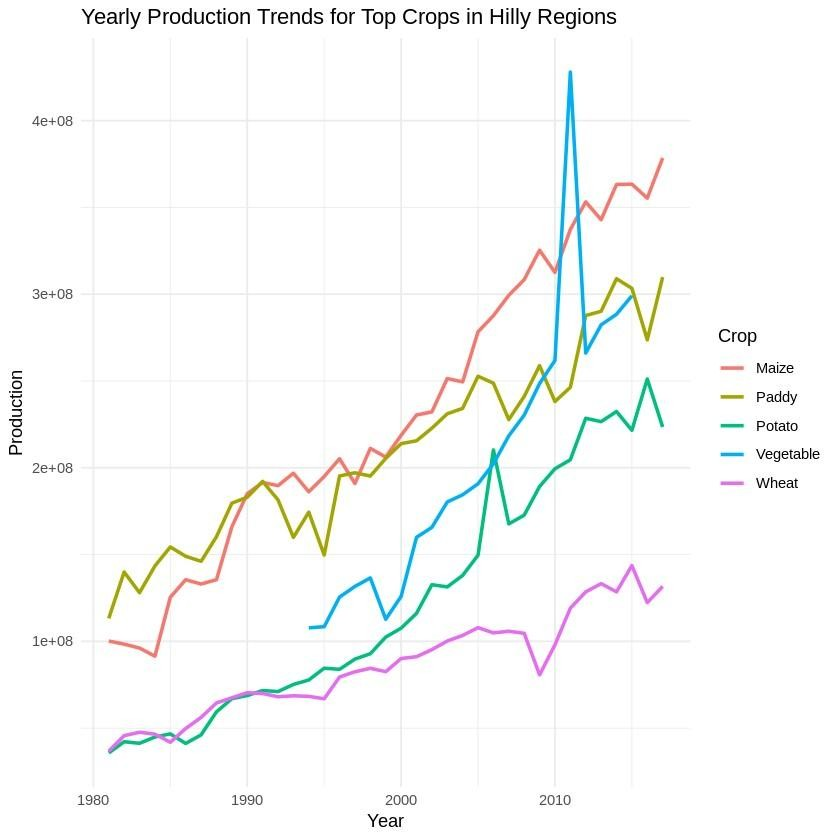
\includegraphics[width=0.5\textwidth]{figures/top5_agri.jpg}
\caption{Trend analysis of Top 5 crops in Hilly}
\end{figure}

\subsection*{Yearly Production of Paddy and Precipitation Trend}

To explore the relationship between agricultural production and climate, we analyze the yearly production of Paddy alongside average precipitation. The following R code aggregates yearly Paddy production and climate data, then plots them with dual y-axes to visualize trends concurrently.

\begin{verbatim}
# Assuming df_paddy_yearly is already created:
df_paddy_yearly <- merged_data %>%
  filter(Crop == "Paddy") %>%
  group_by(Year) %>%
  summarise(
    total_production = sum(Production, na.rm = TRUE),
    avg_temperature = mean(Temp_2m, na.rm = TRUE),
    avg_precip = mean(Precip, na.rm = TRUE)
  )


# Get the max values for dynamic scaling
max_prod_val <- max(df_paddy_yearly$total_production, na.rm = TRUE)
max_precip_val <- max(df_paddy_yearly$avg_precip, na.rm = TRUE)


target_max_proportion <- 0.7


ggplot(df_paddy_yearly, aes(x = Year)) +
  # Line and points for Production
geom_line(aes(y = total_production, color = "Total Production (Kg)"), 
linewidth = 1.2) +
geom_point(aes(y = total_production, color = "Total Production (Kg)"),
size = 3) +

# Line for Precipitation, scaled using the adjusted proportion
geom_line(aes(
  y = avg_precip * (target_max_proportion * max_prod_val / max_precip_val),
  color = "Average Precipitation (mm)"), linewidth = 1.2) +


# Add second axis for Precipitation, using the inverse of the adjusted scaling
scale_y_continuous(
  name = "Total Production (Kg)",
  sec.axis = sec_axis(~ . * (max_precip_val /
   (target_max_proportion * max_prod_val)),name = "Average Precipitation (mm)")
  ) +
# Manually set colors for the lines and define legend labels
scale_color_manual(
  name = "Variable",
  values = c(
      "Total Production (Kg)" = "darkgreen",
      "Average Precipitation (mm)" = "red"
    )
) +
# Titles and labels
labs(
    title = "Yearly Production of Paddy with Precipitation Trend",
    x = "Year"
  ) +
theme_minimal() +
theme(
    axis.text.x = element_text(angle = 45, hjust = 1),
    axis.title.y.left = element_text(color = "darkgreen"),
    axis.title.y.right = element_text(color = "red"),
    legend.position = "bottom",
    legend.title = element_blank(),
    plot.title = element_text(hjust = 0.5, face = "bold")
  )
\end{verbatim}

% Figure here-----------------------------
\begin{figure}[h]
\centering
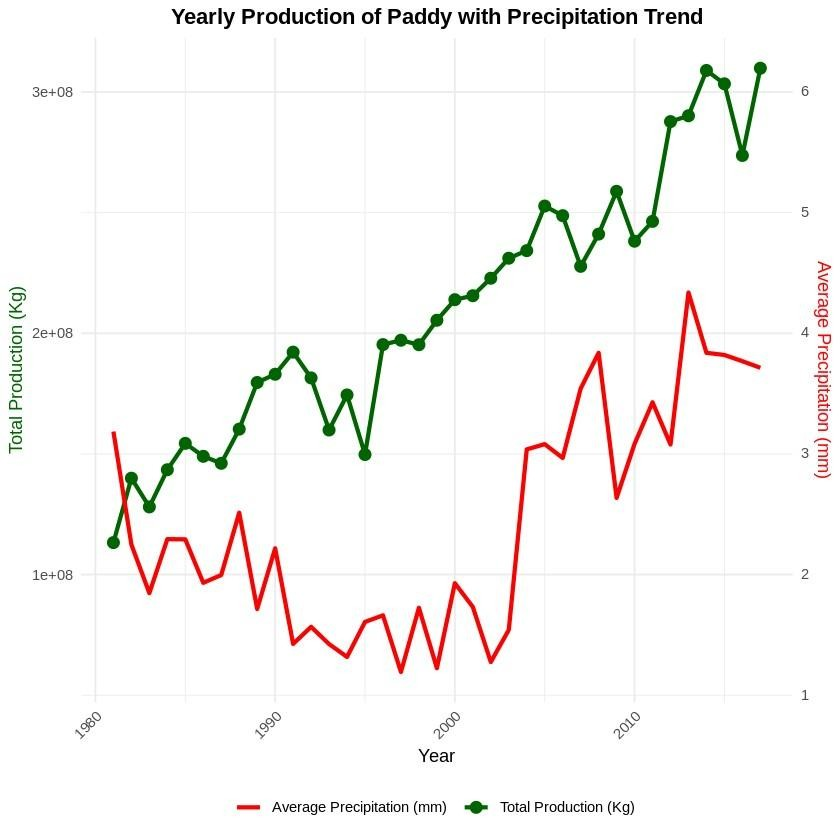
\includegraphics[width=0.5\textwidth]{figures/paddy_trend.jpg}
\caption{Yearly Production of Paddy and Precipitation Trend}
\end{figure}

This plot illustrates how Paddy production varies over the years alongside changes in average precipitation, providing insight into the dependency of agricultural yields on climatic factors in Nepal’s hilly regions. Paddy production has steadily increased over the years, but rainfall shows high variability. Notably, drops in rainfall often correspond to declines in paddy production, highlighting the critical role of adequate rainfall for consistent harvests despite improvements in farming practices.

\subsection*{Correlation Heatmap}

To better understand how climatic factors relate to agricultural outcomes such as crop yield and production, we analyze the correlations between key climate variables and agricultural metrics. This helps reveal any direct linear relationships and the strength of connections within the climate variables themselves. The following code computes and visualizes these correlations using a heatmap.

\begin{verbatim}
library(dplyr)
library(corrplot)
# Step 1: Create a clean numeric dataset for correlation
climate_agri_subset <- aggregated_data %>%
select(avg_temperature, avg_precip, avg_humidity, avg_pressure, avg_wind,
Yield, Production)

# Step 2: Compute correlation matrix
cor_matrix <- cor(climate_agri_subset, use = "complete.obs")

# Step 3: Visualize using corrplot
corrplot(cor_matrix, method = "color",
         type = "upper",        # Only upper triangle
         tl.col = "black",      # Text label color
         addCoef.col = "black", # Add correlation values
         number.cex = 0.7,      # Size of numbers
         col = colorRampPalette(c("red", "white", "blue"))(200))
\end{verbatim}

% Figure here-----------------------------
\begin{figure}[h]
\centering
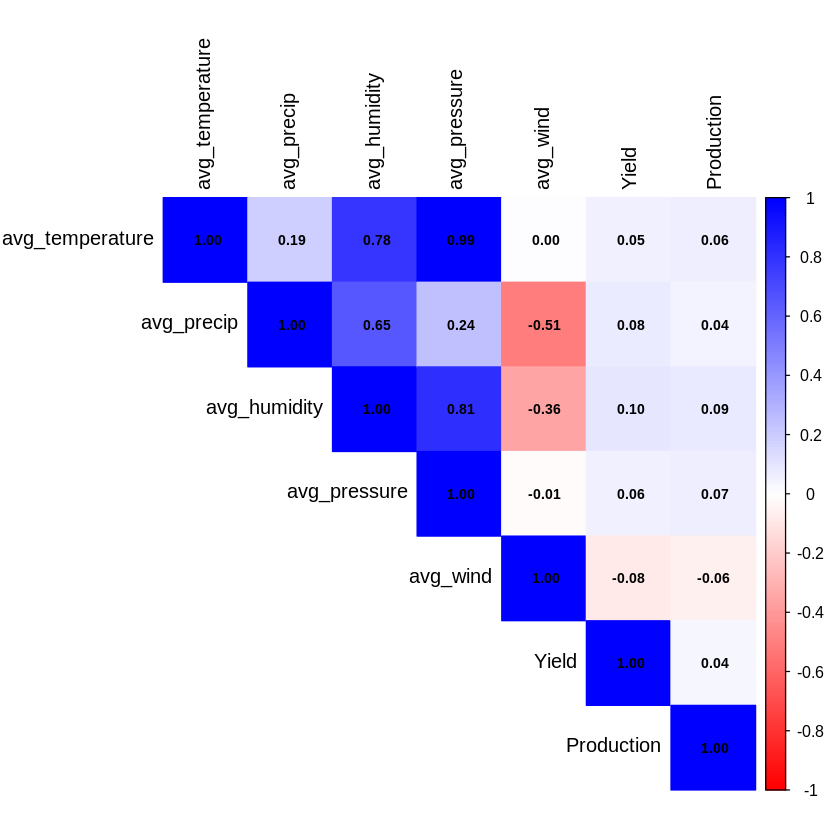
\includegraphics[width=0.5\textwidth]{figures/corr_agri.png}
\caption{Correlation Analysis}
\end{figure}

From this heatmap, several interesting points emerge:

\textbf{Weak Direct Link to Yield and Production:}  
  Correlations between Yield/Production and climate variables (temperature, precipitation, humidity, pressure, wind) are near zero, indicating little to no linear relationship at the annual average level.
  
 \textbf{Why This Matters:}  
 \begin{itemize}
  \item Linear correlation misses non-linear effects (e.g., too much or too little rain affecting yield).  
  \item Annual averages may mask critical seasonal or extreme weather impacts.  
  \item Other factors like technology or irrigation might overshadow climate effects.
 \end{itemize}

 \textbf{Strong Climate Variable Relationships:}  
 \begin{itemize}
  \item Temperature and Pressure: Nearly perfect positive correlation (0.99), suggesting redundancy.  
  \item Humidity: Positively correlated with temperature (0.78) and precipitation (0.65), reflecting natural atmospheric moisture dynamics.  
  \item Wind and Precipitation: Moderately negatively correlated (-0.51), meaning windy years tend to be drier.
 \end{itemize}




